\documentclass[12pt, a4paper]{article}

% ── Pacotes ───────────────────────────────────────────────────────────────────
\usepackage[utf8]{inputenc}
\usepackage[T1]{fontenc}
\usepackage[brazilian]{babel}
\usepackage{colortbl}
\usepackage{geometry}
\usepackage{graphicx}
\usepackage{booktabs}
\usepackage{longtable}
\usepackage{array}
\usepackage{xcolor}
\usepackage{fancyhdr}
\usepackage{titlesec}
\usepackage{pgfplots}
\usepackage{pgfplotstable}
\usepackage{caption}
\usepackage{float}
\usepackage{hyperref}
\usepackage{amsmath}
\usepackage{microtype}
\usepackage{lmodern}

\pgfplotsset{compat=1.18}

% ── Layout ────────────────────────────────────────────────────────────────────
\geometry{
  top=3cm, bottom=2.5cm,
  left=3cm, right=2cm,
  headheight=3cm
}

% ── Cores ─────────────────────────────────────────────────────────────────────
\definecolor{azulescuro}{RGB}{0, 51, 102}
\definecolor{cinzaclaro}{RGB}{240, 240, 240}
\definecolor{vermelho}{RGB}{192, 0, 0}
\definecolor{azul}{RGB}{0, 102, 204}

% ── Cabeçalho e Rodapé ────────────────────────────────────────────────────────
\pagestyle{fancy}
\fancyhf{}
\fancyhead[L]{%
  \raisebox{-0.8cm}{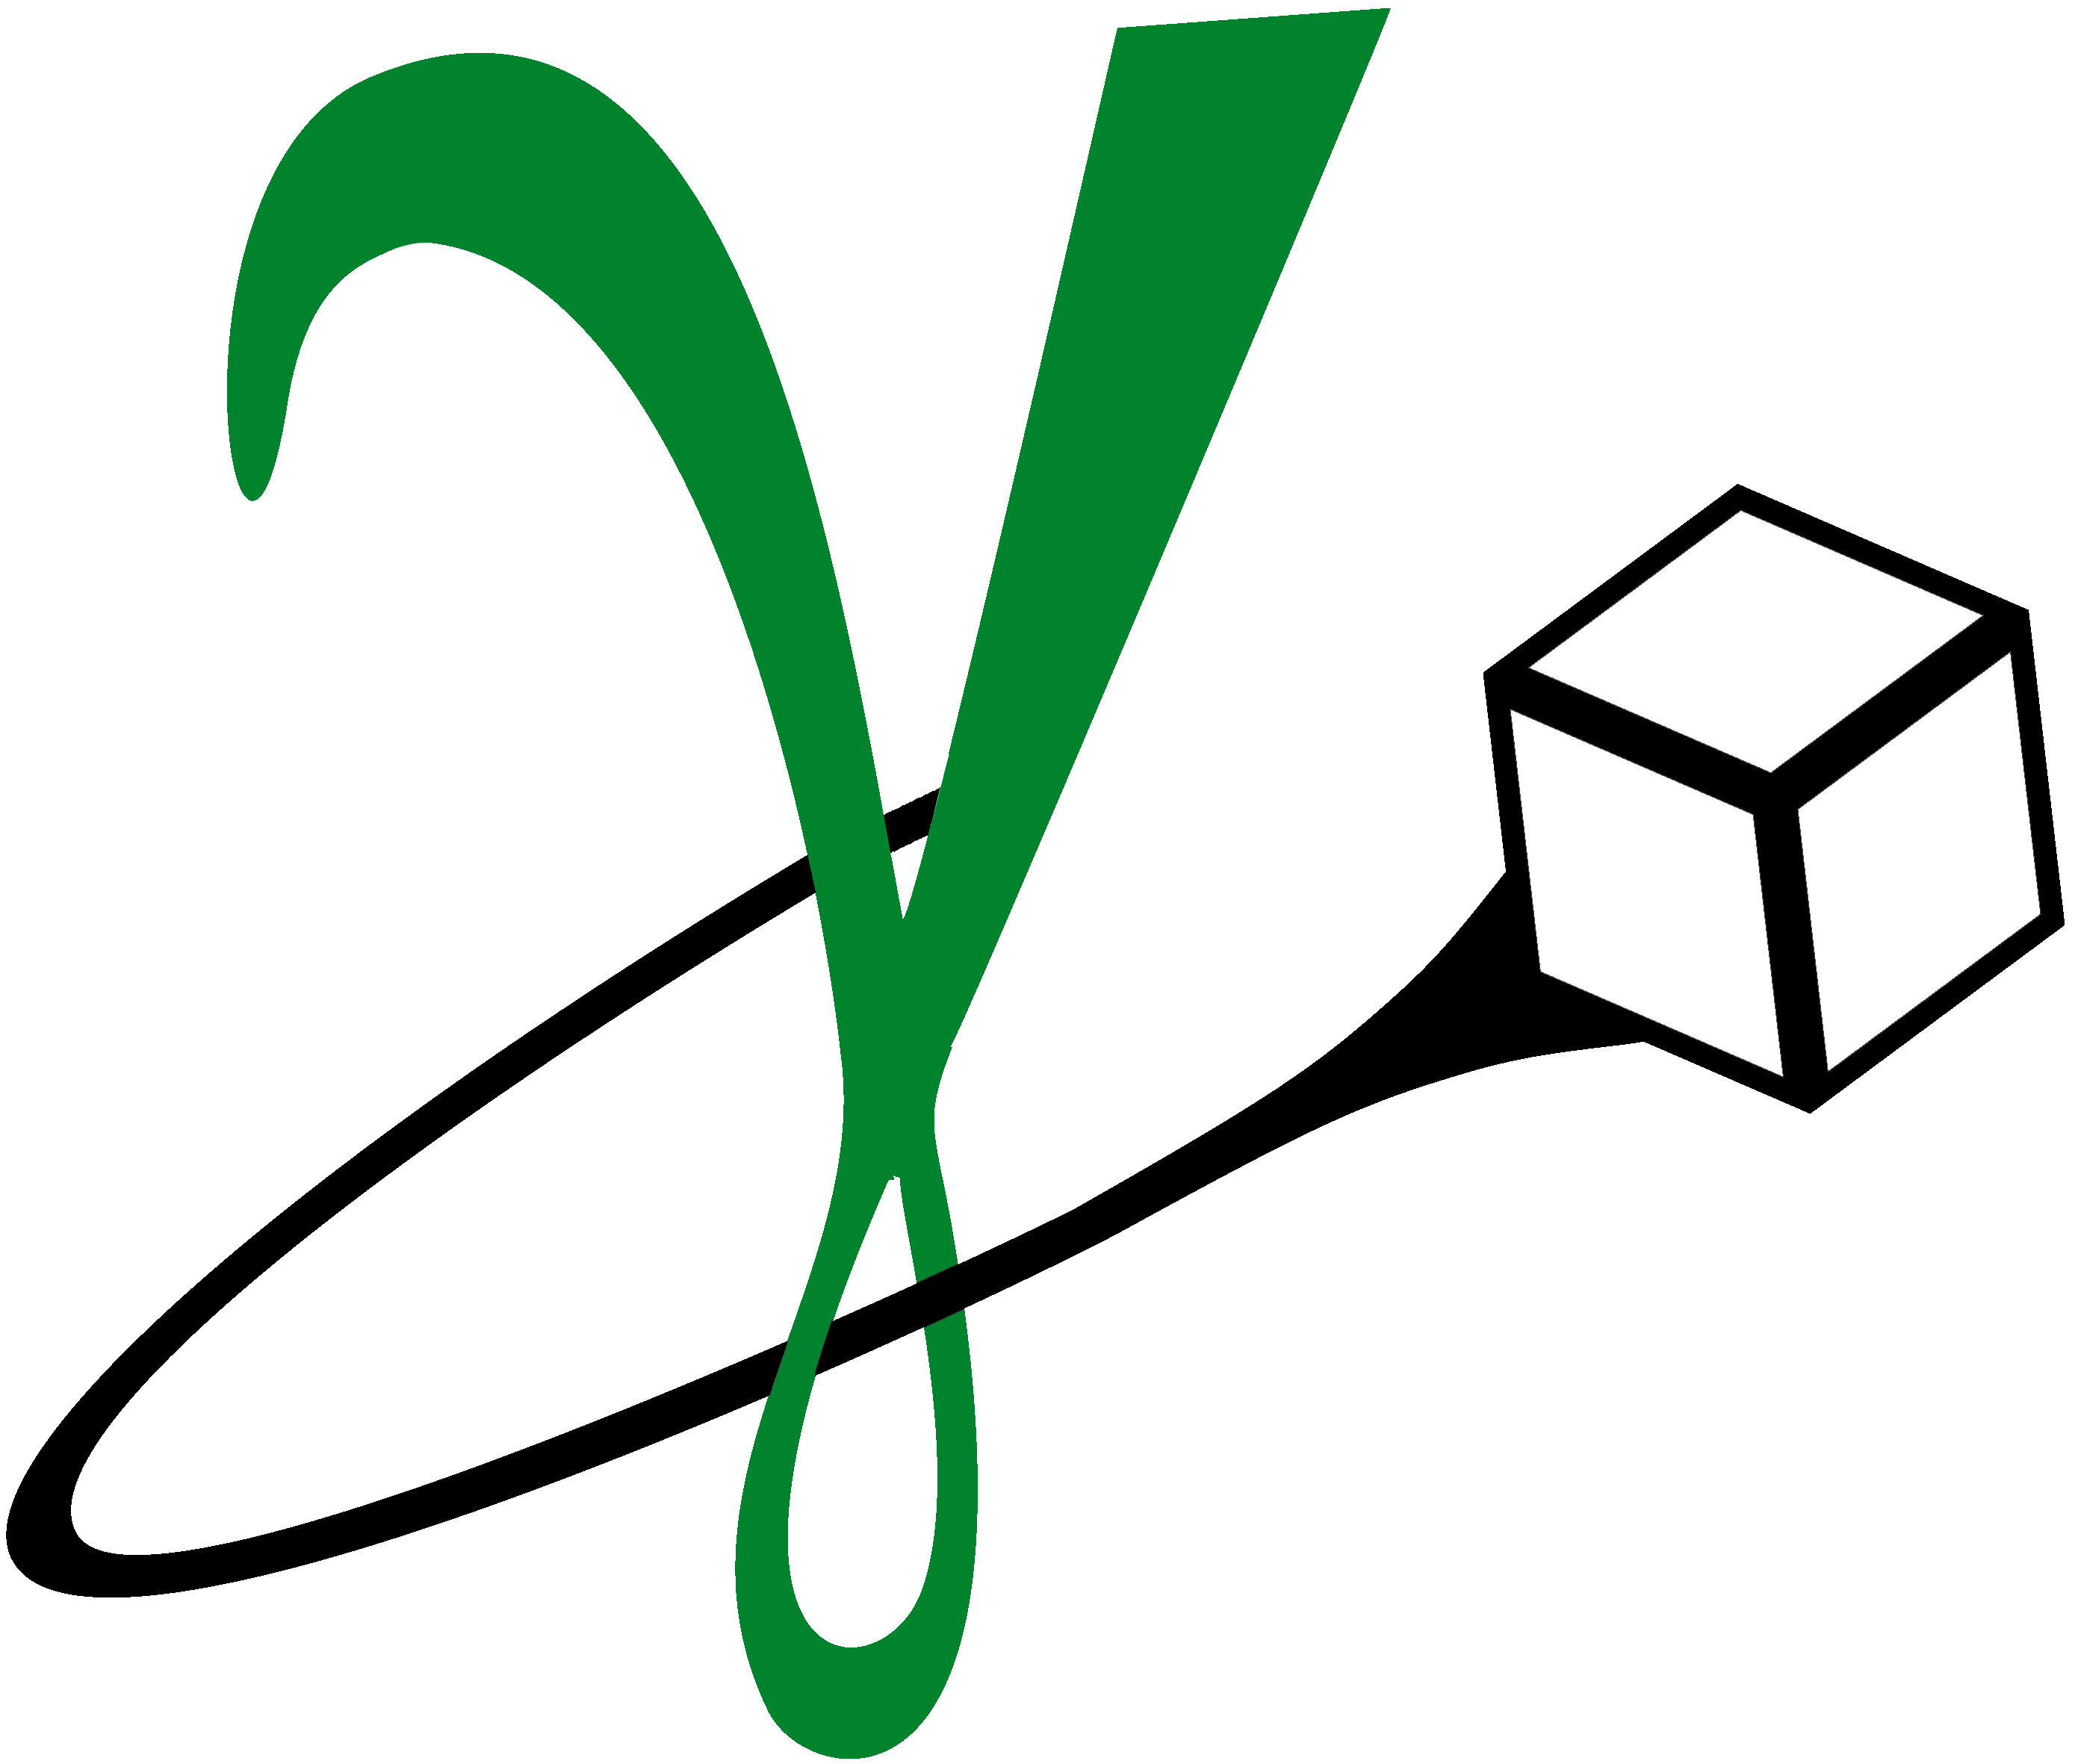
\includegraphics[height=1.8cm]{assets/logo_gama.png}}
}
\fancyhead[C]{%
  \begin{minipage}{0.5\textwidth}
    \centering
    {\small\bfseries Relatório Técnico}\\[2pt]
    {\footnotesize Controle Térmico}
  \end{minipage}
}
\fancyhead[R]{%
  \begin{minipage}{0.25\textwidth}
    \raggedleft
    {\footnotesize\color{gray}
      <<DOC_NUMBER>>\\
      <<DOC_DATE>>\\
    }
  \end{minipage}
}

\fancyfoot[L]{\footnotesize\color{black} Documento Confidencial}
\fancyfoot[C]{\footnotesize\color{black} \thepage}
\fancyfoot[R]{\footnotesize\color{black} Gama CubeDesign}
\renewcommand{\headrulewidth}{0.6pt}
\renewcommand{\footrulewidth}{0.4pt}

% ── Títulos de seção ──────────────────────────────────────────────────────────
\titleformat{\section}
  {\large\bfseries}
  {\thesection.}{0.5em}{}[\titlerule]

\titleformat{\subsection}
  {\normalsize\bfseries}
  {\thesubsection.}{0.5em}{}

% ── Dados pgfplots (injetados pelo Python) ────────────────────────────────────
\pgfplotstableread[col sep=comma]{%
t,ti,te
<<PGFPLOT_DATA>>
}\datatable

% ══════════════════════════════════════════════════════════════════════════════
\begin{document}

% ── Capa ──────────────────────────────────────────────────────────────────────
\thispagestyle{empty}
\begin{titlepage}
  \centering

  \begin{figure}[h]
    \centering
    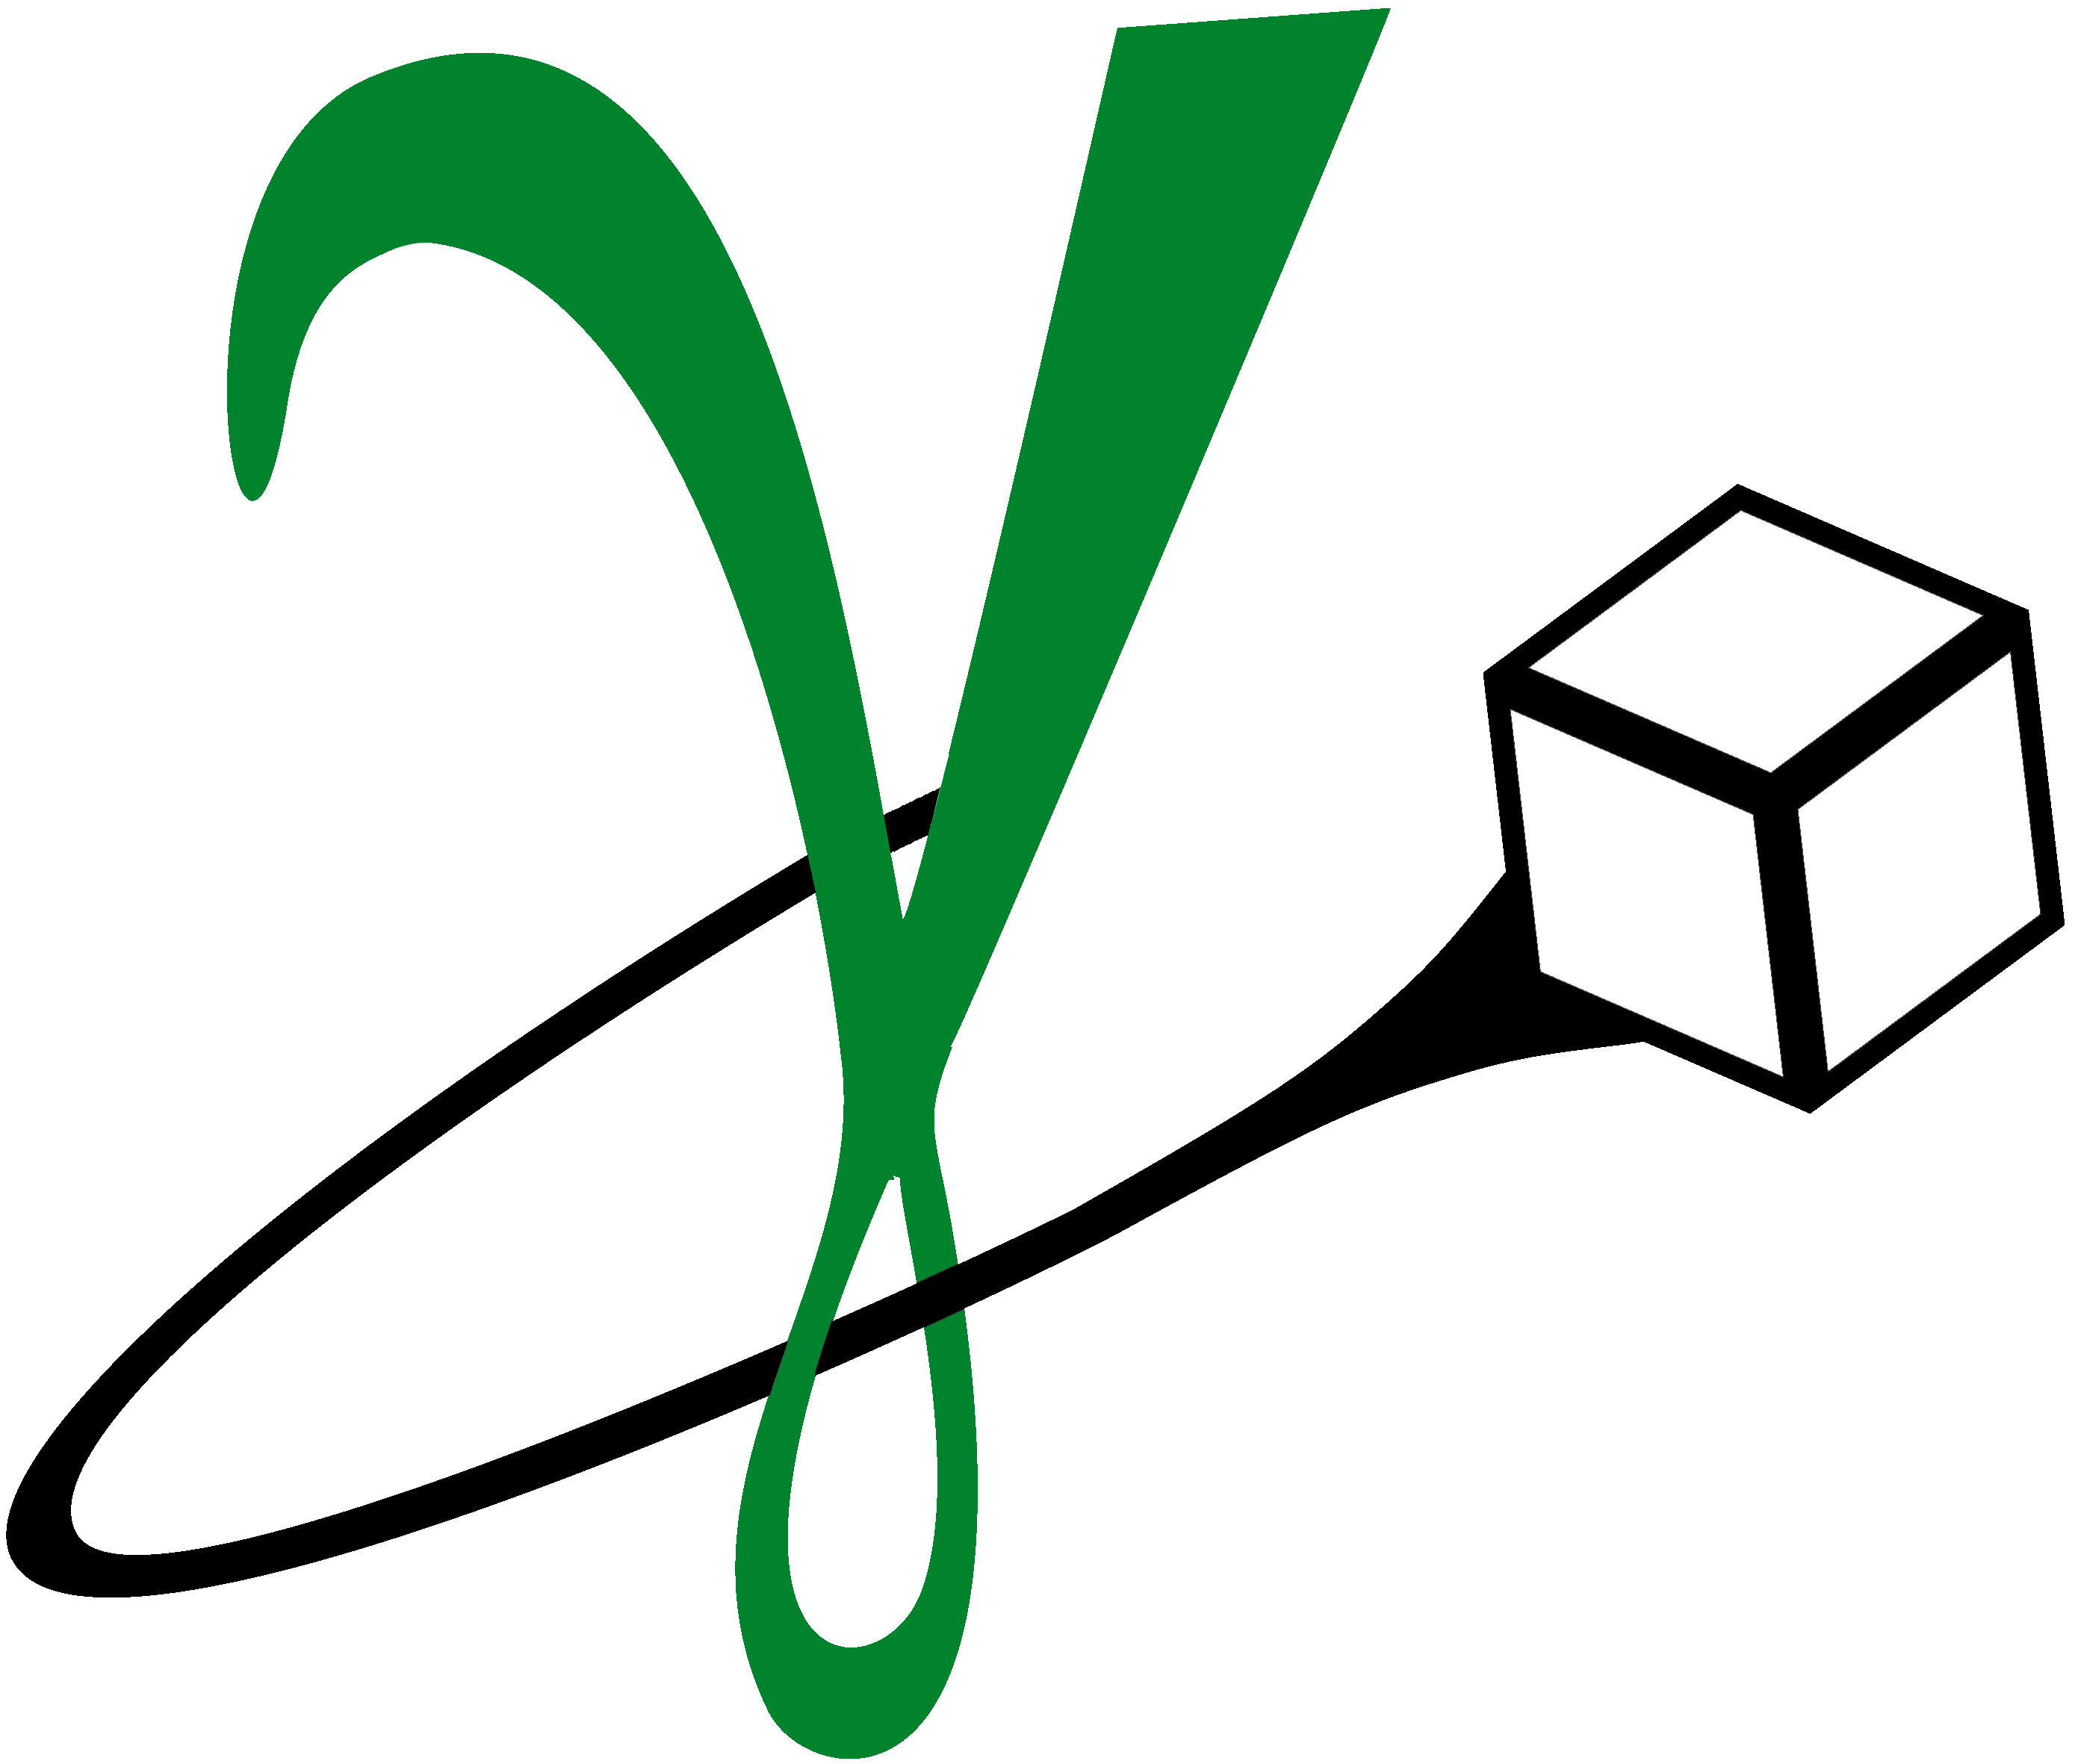
\includegraphics[width=0.5\linewidth]{assets/logo_gama.png}
  \end{figure}

  \vspace{2cm}
  {\Huge\bfseries\color{azulescuro} Relatório Técnico}\\[0.3cm]
  {\Large\color{azulescuro} Controle Térmico}\\[0.1cm]

  \vspace{1.5cm}
  \begin{tabular}{ll}
    \textbf{Documento N.º:}   & <<DOC_NUMBER>> \\[4pt]
    \textbf{Data do Ensaio:}  & <<DOC_DATE_LONG>> \\[4pt]
    \textbf{Status:}          & \textcolor{vermelho}{\textbf{Confidencial}} \\
  \end{tabular}

  \vfill
  {\small\color{gray} Este documento é de uso interno e não deve ser distribuído sem autorização.}
\end{titlepage}

% ── Sumário ───────────────────────────────────────────────────────────────────
\newpage
\tableofcontents
\newpage

% ══════════════════════════════════════════════════════════════════════════════
\section{Objetivo}

Este relatório tem como objetivo apresentar os resultados obtidos durante o ensaio de monitoramento de temperatura realizado em <<DOC_DATE_LONG>>. Foram registradas as temperaturas interna e externa do equipamento em intervalos regulares, durante um período total de <<TEMPO_TOTAL>>, a fim de avaliar o comportamento térmico do sistema sob condições reais de operação.

% ══════════════════════════════════════════════════════════════════════════════
\section{Metodologia}

O ensaio foi conduzido com o equipamento em regime de plena carga. Sensores do tipo ### foram utilizados para aquisição da temperatura interna e externa.

\subsection{Condições do Ensaio}

\begin{itemize}
  \item \textbf{Data/hora de início:} <<TIMESTAMP_INICIO>>
  \item \textbf{Data/hora de término:} <<TIMESTAMP_FIM>>
  \item \textbf{Duração total:} <<TEMPO_TOTAL>>
  \item \textbf{Total de registros:} <<TOTAL_SAMPLES>> amostras
  \item \textbf{Sensor interno:} ### --- Precisão ±0{,}1\,°C
  \item \textbf{Sensor externo:} ### --- Precisão ±0{,}1\,°C
\end{itemize}

% ══════════════════════════════════════════════════════════════════════════════
\section{Resultados}

\subsection{Tabela de Temperaturas}

A Tabela~\ref{tab:temperaturas} apresenta todos os valores de temperatura registrados durante o ensaio.

\begin{longtable}{%
  >{\centering\arraybackslash}m{1.2cm}
  >{\centering\arraybackslash}m{5.2cm}
  >{\centering\arraybackslash}m{3.5cm}
  >{\centering\arraybackslash}m{3.5cm}
}
\caption{Temperaturas interna e externa registradas durante o teste.}
\label{tab:temperaturas}\\
\toprule
\rowcolor{azulescuro}
\textcolor{white}{\textbf{\#}} &
\textcolor{white}{\textbf{Timestamp}} &
\textcolor{white}{\textbf{Temp.\ Interna (°C)}} &
\textcolor{white}{\textbf{Temp.\ Externa (°C)}} \\
\midrule
\endfirsthead

\multicolumn{4}{c}{\footnotesize\itshape (continuação da Tabela~\ref{tab:temperaturas})}\\
\toprule
\rowcolor{azulescuro}
\textcolor{white}{\textbf{\#}} &
\textcolor{white}{\textbf{Timestamp}} &
\textcolor{white}{\textbf{Temp.\ Interna (°C)}} &
\textcolor{white}{\textbf{Temp.\ Externa (°C)}} \\
\midrule
\endhead

\bottomrule
\endfoot

\bottomrule
\endlastfoot

<<TABLE_DATA>>

\end{longtable}

% ── Resumo Estatístico ────────────────────────────────────────────────────────
\subsection{Resumo Estatístico}

\begin{table}[H]
  \centering
  \caption{Estatísticas descritivas das temperaturas registradas.}
  \label{tab:stats}
  \begin{tabular}{lcc}
    \toprule
    \textbf{Parâmetro} & \textbf{Temp.\ Interna (°C)} & \textbf{Temp.\ Externa (°C)} \\
    \midrule
    Mínima   & <<MIN_INTERNA>>  & <<MIN_EXTERNA>>  \\
    Máxima   & <<MAX_INTERNA>>  & <<MAX_EXTERNA>>  \\
    Média    & <<MEDIA_INTERNA>> & <<MEDIA_EXTERNA>> \\
    Variação & <<VAR_INTERNA>>  & <<VAR_EXTERNA>>  \\
    \bottomrule
  \end{tabular}
\end{table}

% ── Gráfico ───────────────────────────────────────────────────────────────────
\subsection{Gráfico de Temperatura $\times$ Tempo}

A Figura~\ref{fig:grafico} ilustra a evolução das temperaturas interna e externa ao longo do ensaio.

\begin{figure}[H]
  \centering
  \begin{tikzpicture}
    \begin{axis}[
      width=0.92\textwidth,
      height=8cm,
      xlabel={Tempo (min)},
      ylabel={Temperatura (°C)},
      xmin=<<XMIN>>, xmax=<<XMAX>>,
      ymin=<<YMIN>>, ymax=<<YMAX>>,
      grid=both,
      grid style={line width=0.3pt, draw=gray!30},
      major grid style={line width=0.5pt, draw=gray!50},
      legend pos=outer north east,
      legend style={font=\small},
      tick label style={font=\small},
      label style={font=\small\bfseries},
      title style={font=\normalsize\bfseries\color{azulescuro}},
      title={Evolução Térmica --- Ensaio de <<DOC_DATE>>},
      axis background/.style={fill=gray!5},
    ]

    \addplot[
      color=azul,
      line width=1.8pt,
      mark=*,
      mark size=2pt,
    ] table[x=t, y=ti, col sep=comma] \datatable;
    \addlegendentry{Temp.\ Interna}

    \addplot[
      color=vermelho,
      line width=1.8pt,
      mark=square*,
      mark size=2pt,
      dashed,
    ] table[x=t, y=te, col sep=comma] \datatable;
    \addlegendentry{Temp.\ Externa}

    \end{axis}
  \end{tikzpicture}
  \caption{Temperaturas interna (azul) e externa (vermelho) em função do tempo de ensaio.}
  \label{fig:grafico}
\end{figure}

\end{document}